\subsection{Computational domain and discrete grid}
From this point forward $ \Delta l $ and $ \Delta t $ represent non-dimensional spatial and time step, respectively. We consider a cuboidal computational domain $ \Omega \subset \mathbb{R}^3 $, see Section~ \ref{pred}. This domain is discretized using an equidistant grid

\begin{subequations}\label{eq:domain}
	\begin{eqnarray}
		&\hat{\Omega} = \left\{ \vec{x}_{i,j,k} = (i \Delta l,\,j \Delta l, \,k \Delta l)^T \ \middle| \ i \in \{1, \dots, N_{1} - 1\}, j \in \{1, \dots, N_{2} - 1 \}, k \in \{1, \dots, N_{3} - 1 \} \right\},\\[4pt]
		&\overline{\hat{\Omega}} = \left\{ \vec{x}_{i,j} = (i \Delta l,\,j \Delta l)^T \ \middle| \ i \in \{0, \dots, N_{1} \}, j \in \{0, \dots, N_{2} \}, k \in \{0, \dots, N_{3} \} \right\},
	\end{eqnarray}
\end{subequations}
where $ N_{i} $ [-] denotes the number of grid points in the $ x_i $ direction, $ i = 1, 2, 3 $.

The boundary of the domain $ \Omega $ is denoted by $ \partial \Omega $ and is defined as the closure of the union of disjoint parts 
\begin{equation}\label{eq:border decomposition}
	\partial \Omega = \overline{\partial \Omega_{\mathrm{W}} \cup \partial \Omega_{\mathrm{E}} \cup \partial \Omega_{\mathrm{N}} \cup \partial \Omega_{\mathrm{S}} \cup \partial \Omega_{\mathrm{F}} \cup \partial \Omega_{\mathrm{B}}},
\end{equation}
where $\partial \Omega_{\mathrm{W}} , \partial \Omega_{\mathrm{E}} , \partial \Omega_{\mathrm{N}}, \partial \Omega_{\mathrm{S}}, \partial \Omega_{\mathrm{F}}$, and $  \partial \Omega_{\mathrm{B}} $ represent the west, east, north, south, front, and back boundaries, respectively, as illustrated in~Figure \ref{fig:domain}. The discretized boundary of the computational domain is given by
\begin{equation}\label{eq:border}
	\partial\hat{\Omega} = \overline{\hat{\Omega}} \, \backslash \, \hat{\Omega},
\end{equation}
with its corresponding parts denoted by $ \partial \hat{\Omega}_{\mathrm{W}} , \partial \hat{\Omega}_{\mathrm{E}} , \partial \hat{\Omega}_{\mathrm{N}}, \partial \hat{\Omega}_{\mathrm{S}}, \partial \hat{\Omega}_{\mathrm{F}}$,  and $ \partial \hat{\Omega}_{\mathrm{B}} $.
\begin{figure}[H]
	\centering
	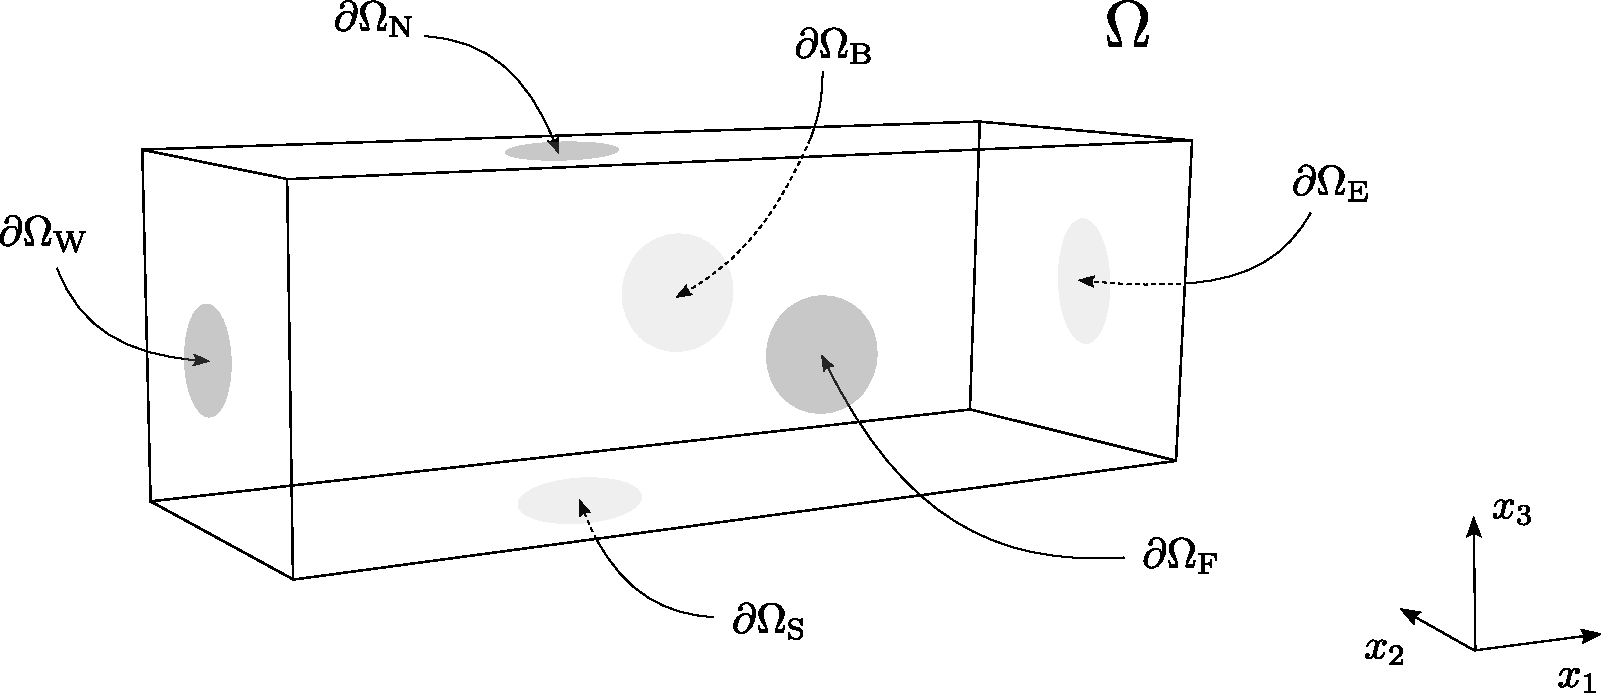
\includegraphics[width=0.99\textwidth]{figures/omega.pdf}
	\caption{Schematic representation of the computational domain $ \Omega $ and its boundary $ \partial \Omega $.}  
	\label{fig:domain}
	\vspace{1.8mm}
\end{figure}

The time interval of interest is denoted by $ \mathcal{I} $ , where ${\mathcal{I} = [ 0, T ]}$, and $ T > 0 $. The interval $ \mathcal{I} $ is discretized as
\begin{equation}\label{eq:timediscrete}
	\hat{\mathcal{I}} = \left\{ t_{i} = i \frac{T}{N_t} \ \middle| \ i \in \left\{0, \dots, N_{t} \right\} \right\},
\end{equation}
where $ N_t $ represents the number of discrete time steps.

\subsection{Discrete Boltzmann transport equation}
When using the D3Q27 model, we work with a set of distribution functions
\begin{equation}\label{eq:ddfs}
	\left\{ f_k (\vec{x}, t) \ \middle| \ k = 1, \dots, 27 \right\}, \ \forall \vec{x} \in \hat{\Omega}, \ \forall t \in \hat{\mathcal{I}},
\end{equation}
where the indices correspond to the directions of microscopic velocities from \eqref{eq:velocities}.

It can be shown that by discretizing the equation \eqref{eq:BTR}, we obtain the form
\begin{equation}\label{eq:BTRdiscrete}
	f_{k}\left(\vec{x}+\Delta t \vec{\xi}_{k}, t+\Delta t \right) =
	f_{k}(\vec{x}, t) + \mathcal{C}_{k}(\vec{x}, t) + \mathcal{S}_{k}(\vec{x}, t), \hspace{2.5mm} k \in \{1, \dots, 27 \}, \ \forall \vec{x} \in \hat{\Omega}, \ \forall t \in \hat{\mathcal{I}},
\end{equation}
where $ \mathcal{C}_{k} $ represents the discrete collision operator, and $ \mathcal{S}_{k} $ is the discrete forcing term. Details of the derivation can be found in \cite{Kruger}.

The choice of the discrete collision operator $\mathcal{C}_{k}$ in equation \eqref{eq:BTRdiscrete} defines the specific variant of LBM. Several choices for $\mathcal{C}_{k}$ exist, including single relaxation time (SRT-LBM) \cite{GeierCuLBM}, multiple relaxation time (MRT-LBM) \cite{MRT}, central moment (CLBM) \cite{GeierCLBM}, entropic (ELBM) \cite{ELBM}, and cumulant-based (CuLBM) \cite{GeierCuLBM}. In this work, we use the cumulant collision operator, as detailed in \cite{GeierCuLBM}.

To simplify the computation of the discrete equation, we define the post-collision distribution functions $ f^{*}_{k} $ as
\begin{equation}\label{eq:fstar}
	f^{*}_{k}(\vec{x}, t) = f_{k}(\vec{x}, t) + \mathcal{C}_{k}(\vec{x}, t) + \mathcal{S}_{k}(\vec{x}, t), \hspace{2.5mm} k \in \{1, \dots, 27 \}, \ \forall \vec{x} \in \hat{\Omega}, \ \forall t \in \hat{\mathcal{I}}.
\end{equation}
Using $ f^{*}_{k} $, we can express \eqref{eq:BTRdiscrete} in the form
\begin{equation}\label{eq:collision}
	f_{k}\left(\vec{x}+\Delta t \vec{\xi}_{k}, t+\Delta t\right) = f^{*}_{k}(\vec{x}, t), \hspace{2.5mm} k \in \{1, \dots, 27 \}, \ \forall \vec{x} \in \hat{\Omega}, \ \forall t \in \hat{\mathcal{I}}.
\end{equation}
This formulation allows for an explicit prescription of calculating the distribution functions.